% Applying H to an MPS (contraction + SVD compression) and the DMRG sweep (Session 5).
% Own drawing (Fable). Compile with: pdflatex mps_algorithm.tex ; result moves to ../mps_algorithm.pdf
\documentclass[11pt,tikz,border=3pt]{standalone}
\usepackage{amsmath,amssymb}
\usepackage{xcolor}
\definecolor{coursedark}{HTML}{1B2A4A}
\definecolor{courseaccent}{HTML}{7A2E8C}

\begin{document}
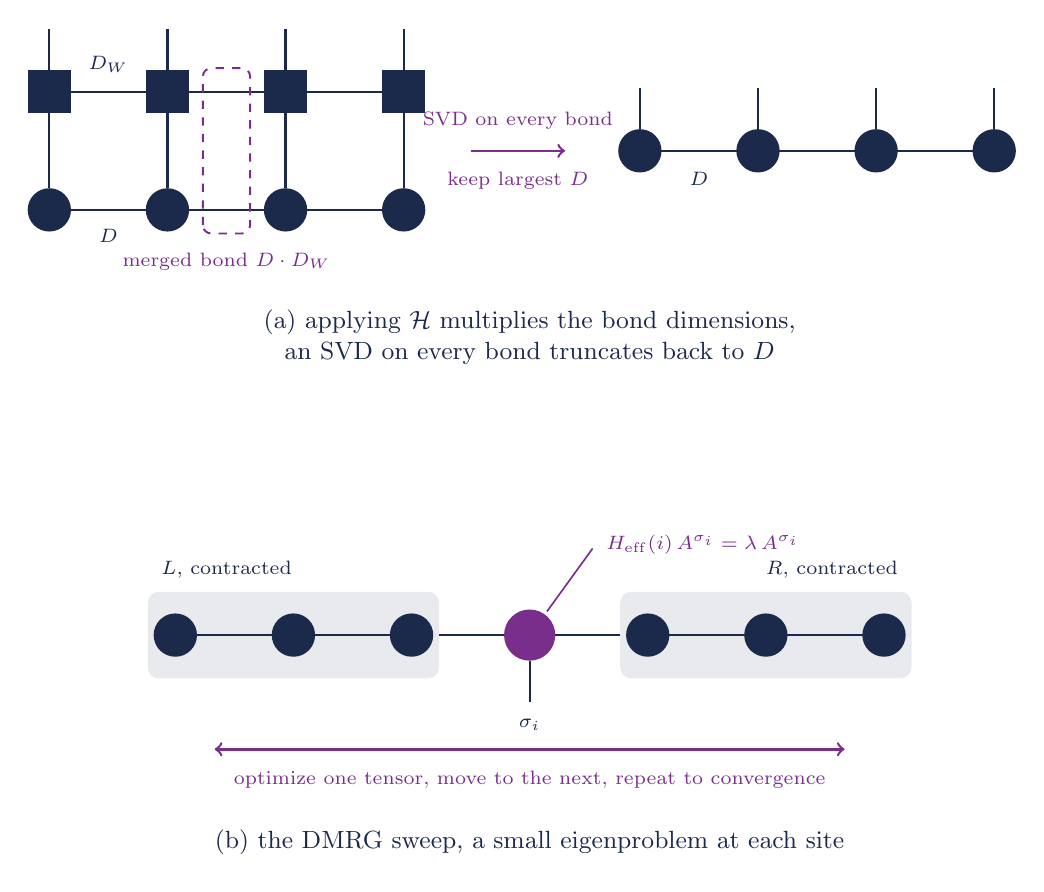
\begin{tikzpicture}[
    mps/.style={circle, fill=coursedark, inner sep=0pt, minimum size=5.5mm},
    mpo/.style={rectangle, fill=coursedark, inner sep=0pt, minimum size=5.5mm},
    active/.style={circle, fill=courseaccent, inner sep=0pt, minimum size=6.5mm},
    wire/.style={draw=coursedark, line width=0.8pt},
    lbl/.style={font=\small, text=coursedark, align=center},
    idx/.style={font=\scriptsize, text=coursedark, align=center},
  ]

  % ================= panel (a): H|Psi>, bond growth, SVD truncation
  \begin{scope}[shift={(0,0)}]
    % MPS row (physical legs point up, joined to the MPO's column legs)
    \foreach \x in {0,1.5,3.0,4.5} { \node[mps] at (\x,0) {}; }
    \draw[wire] (0,0) -- (4.5,0);
    \node[idx, anchor=north] at (0.75,-0.12) {$D$};
    % MPO row
    \foreach \x in {0,1.5,3.0,4.5} { \node[mpo] at (\x,1.5) {}; }
    \draw[wire] (0,1.5) -- (4.5,1.5);
    \node[idx, anchor=south] at (0.75,1.62) {$D_W$};
    % joined physical legs and free output legs
    \foreach \x in {0,1.5,3.0,4.5} {
      \draw[wire] (\x,0.275) -- (\x,1.225);
      \draw[wire] (\x,1.775) -- (\x,2.30);
    }
    % merged-bond highlight between columns 2 and 3
    \draw[courseaccent, dashed, line width=0.7pt, rounded corners=3pt]
      (1.95,-0.30) rectangle (2.55,1.80);
    \node[idx, text=courseaccent, anchor=north] at (2.25,-0.42) {merged bond $D\cdot D_W$};
    % SVD arrow
    \draw[->, courseaccent, line width=0.9pt] (5.35,0.75) -- (6.55,0.75);
    \node[idx, text=courseaccent, anchor=south] at (5.95,0.90) {SVD on every bond};
    \node[idx, text=courseaccent, anchor=north] at (5.95,0.60) {keep largest $D$};
    % compressed result
    \foreach \x in {7.5,9.0,10.5,12.0} {
      \node[mps] at (\x,0.75) {};
      \draw[wire] (\x,1.025) -- (\x,1.55);
    }
    \draw[wire] (7.5,0.75) -- (12.0,0.75);
    \node[idx, anchor=north] at (8.25,0.60) {$D$};
    \node[lbl, anchor=north] at (6.1,-1.15)
      {(a) applying $\mathcal{H}$ multiplies the bond dimensions,\\
       an SVD on every bond truncates back to $D$};
  \end{scope}

  % ================= panel (b): the DMRG sweep
  \begin{scope}[shift={(1.6,-5.4)}]
    % left environment
    \fill[coursedark!10, rounded corners=4pt] (-0.35,-0.55) rectangle (3.35,0.55);
    \foreach \x in {0,1.5,3.0} { \node[mps] at (\x,0) {}; }
    \draw[wire] (0,0) -- (3.0,0);
    \node[idx, anchor=south west] at (-0.30,0.60) {$L$, contracted};
    % right environment
    \fill[coursedark!10, rounded corners=4pt] (5.65,-0.55) rectangle (9.35,0.55);
    \foreach \x in {6.0,7.5,9.0} { \node[mps] at (\x,0) {}; }
    \draw[wire] (6.0,0) -- (9.0,0);
    \node[idx, anchor=south east] at (9.30,0.60) {$R$, contracted};
    % active site
    \node[active] at (4.5,0) {};
    \draw[wire] (3.35,0) -- (4.175,0);
    \draw[wire] (4.825,0) -- (5.65,0);
    \draw[wire] (4.5,-0.325) -- (4.5,-0.85);
    \node[idx, anchor=north] at (4.5,-0.95) {$\sigma_i$};
    % local eigenproblem annotation, diagonal leader
    \node[idx, text=courseaccent, anchor=west] at (5.35,1.15)
      {$H_{\mathrm{eff}}(i)\,A^{\sigma_i}=\lambda\,A^{\sigma_i}$};
    \draw[courseaccent, line width=0.6pt] (5.30,1.10) -- (4.72,0.30);
    % sweep arrow
    \draw[<->, courseaccent, line width=0.9pt] (0.5,-1.45) -- (8.5,-1.45);
    \node[idx, text=courseaccent, anchor=north] at (4.5,-1.60)
      {optimize one tensor, move to the next, repeat to convergence};
    \node[lbl, anchor=north] at (4.5,-2.35)
      {(b) the DMRG sweep, a small eigenproblem at each site};
  \end{scope}
\end{tikzpicture}
\end{document}
